\documentclass[conference]{IEEEtran}
\IEEEoverridecommandlockouts
% The preceding line is only needed to identify funding in the first footnote. If that is unneeded, please comment it out.
\usepackage{cite}

\usepackage{algorithm}
\usepackage{amsmath}
\usepackage{algpseudocode}
\usepackage{lmodern}
\usepackage{microtype}
\usepackage{amsmath}
\usepackage{mathrsfs}
\usepackage{mathtools}
\usepackage{xcolor}
\usepackage{ulem}
\usepackage{graphicx}
\usepackage{float}
\usepackage{subfigure}

\usepackage[hyphens]{url}
\begin{document}

\title{Gradient Descend\\}

\author{\IEEEauthorblockN{ Luca Brodo}
\IEEEauthorblockA{\textit{Hochschule Hamm-Lippstadt} \\
\textit{Deep Learning}\\
Lippstadt, Germany \\
luca.brodo@stud.hshl.de}
}

\maketitle


\begin{abstract}
The objective of this paper is to give to the reader a thorough overview of the Gradient Descent Algorithm applied in the area of Machine Learning. In this paper the different variations of this algorithm will be introduced and explained. In order to offer a complete understanding, both the mathematical foundations and an application will be presented. This will be used to compare the different algorithms and to show their characteristics.
\end{abstract}


\section{Motivation}
The main challenge in the area of Machine Learning for both researchers and practitioners is to train the model as efficiently as possible. In the context of Deep Neural Network models the training is based on the back propagation algorithm, which propagates the errors from the output layer to the front one, updating the variables layer by layer, and it's based on gradient descent optimization algorithms.A lot of different algorithms have been introduced to better improve the performances of the models,e.g., Newton’s method, but hese algorithms are based on high-order derivatives and in practice tend to be slower than the first-derivative-based Gradient Descent and its variants. 
In the context of linear regression based models, performances play also a major role and an optimized algorithm may result vital when the data set is big. Usually, they are often used as black-box optimizers by state-of-the-art Deep Learning library, e.g. lasagne, caffe, and keras documentation, but an ad-hoc implementation for a specific dataset may be more efficient. To achieve so, a full understanding of the algorithm is necessary. 

\section{Introduction}

The aim of this paper is to provide a thorough understanding of the Gradient Descent algorithm for optimization in the area of Machine Learning. In this section, a first introduction to the algorithm will be provided. Subsequently, in section 2, the mathematical foundations of the algorithm will be layed down. In the next three sections, the three different versions of the algorithm, namely the Batch, Stochastic and Mini-Batch Gradient Descent, are discussed in detail and compared along with a an application.
\\
As already mentioned, the gradient descent is an algorithm that allows the optimization of various machine learning models. In order to achieve this, the algorithm is based on an iterative process for finding a local minima of a differentiable function. At every iteration, the step in the opposite direction of the gradient\footnote{ The gradient represents in which point the function changes the most}  of the function at the given point is taken. 
This algorithm is usually attributed to Cauchy, who first suggested it in 1847.

\subsection{Real World Example}

The above described algorithm can be better visualized with a real world example.
Let's assume a situation in which one finds himself on the top of a mountain and needs to reach the valley. In case the visibility is very low, for example because of extreme fog, one solution can be to walk some steps and to always choose the steepest path. If one keeps going like this, eventually the valley will be reached. 
This is the main idea behind the algorithm. 




\section{Mathematical Foundations}

The algorithm moves from the observation that, taken a multi-variable,defined and differentiable in a point \textbf{a} function $F(x)$, it will decrease fastest whenever one goes from \textbf{a}  towards $-$ $\nabla F(x)$  (opposite to the gradient of $F(x)$).
It follows, then:
\begin{equation}
    \mathbf{a_{n}} = \mathbf{a_{n-1}} - \alpha\nabla F(\mathbf{a_{n-1}})\label{eq:original}
\end{equation}
where $\alpha$ is small enough, so that $F(a_{n-1} \geq a_{n})$.\\\\
In other words, by subtracting $\alpha\nabla F(\mathbf{a_{n-1}})$ to $\mathbf{a_{n-1}}$, one moves against the gradient, towards the local minima as fast as possible. \\By considering each point $\mathbf{a_{0}},\mathbf{a_{1}},\mathbf{a_{2}},...\mathbf{a_{n},\mathbf{a_{n+1}}}$, such that 
$\mathbf{a_{n+1}} = \mathbf{a_{n}} - \alpha\nabla F(\mathbf{a_{n}})$, one will obtain the following monotonic sequence:
\[
   F(a_{0}) \geq F(a_{1})\geq F(a_{2})\geq F(a_{3})\geq F(a_{4}) \geq ...
\]

This sequence will converge to the local minima of the function.\cite{Wikipedia}



\section{Machine Learning Application}


When training a model, a so called "Cost function" is used to express the average loss over the data set.\\
Calculating the slope, or gradient, of this function at a given point defines how the function changes at that point, thus giving insights on how to change the parameters of the model to make it more accurate.By finding the minimum of this function,the perfect value of the parameters that minimizes the cost of the model is found. 
Recalling the previous section, the concept of taking steps opposite to the gradient has been introduced. These steps, in the context of machine learning, are called "learning rate".
Choosing the correct value for the learning rate will produce a behavior like the one shown in Fig \ref{fig:normalbeh},where the minimum of the function is found. \\
On the other hand, choosing an improper value for the steps will introduce imprecision or it will slow down the process.
Recalling the real world example again, let's imagine that the person on the mountain had with them a tool capable of measuring the steepness of the mountain at a specific point. \\
By walking too much in one direction, it may be the case that the value measured at the destination point is bigger that the one measured at the starting point. This is referred as overshooting in machine learning and it's visualized in Fig n.\ref{fig:first}. Basically, the value will increase instead of decreasing if a big value for the learning rate is chosen.\\
However, if the person uses the tool too many times,i.e. chooses a very small learning rage, the process will be slowed down by the time taken by the tool to calculate, as shown in Fig n.\ref{fig:second} \footnote{ The steps are not far enough and the algorithm is stuck in a plateau}.. In other words, while using close steps is more precise, it also introduces calculation overhead, since the gradient is recalculated very frequently, thus making the learning process slower. \cite{Scikit-Learn}\\
Finally, not all cost functions will be nice, smooth parabolas like the ones shown in the previous pictures. This means that, instead of the local minimum, the gradient descent might stop at one local, which is not as idea as the global minimum, like in Fig n.\ref{fig:pitfallsbeh} .\cite{Scikit-Learn} . 
To solve this problem, a cost function without local minimas should be used. To insure so, the Rolle Theorem can be used\cite{Roll}. For the scope of this paper, the Mean Squared Error (MSE) cost function will be used and it has been proven not to have local minimas



\begin{figure}[htbp]
    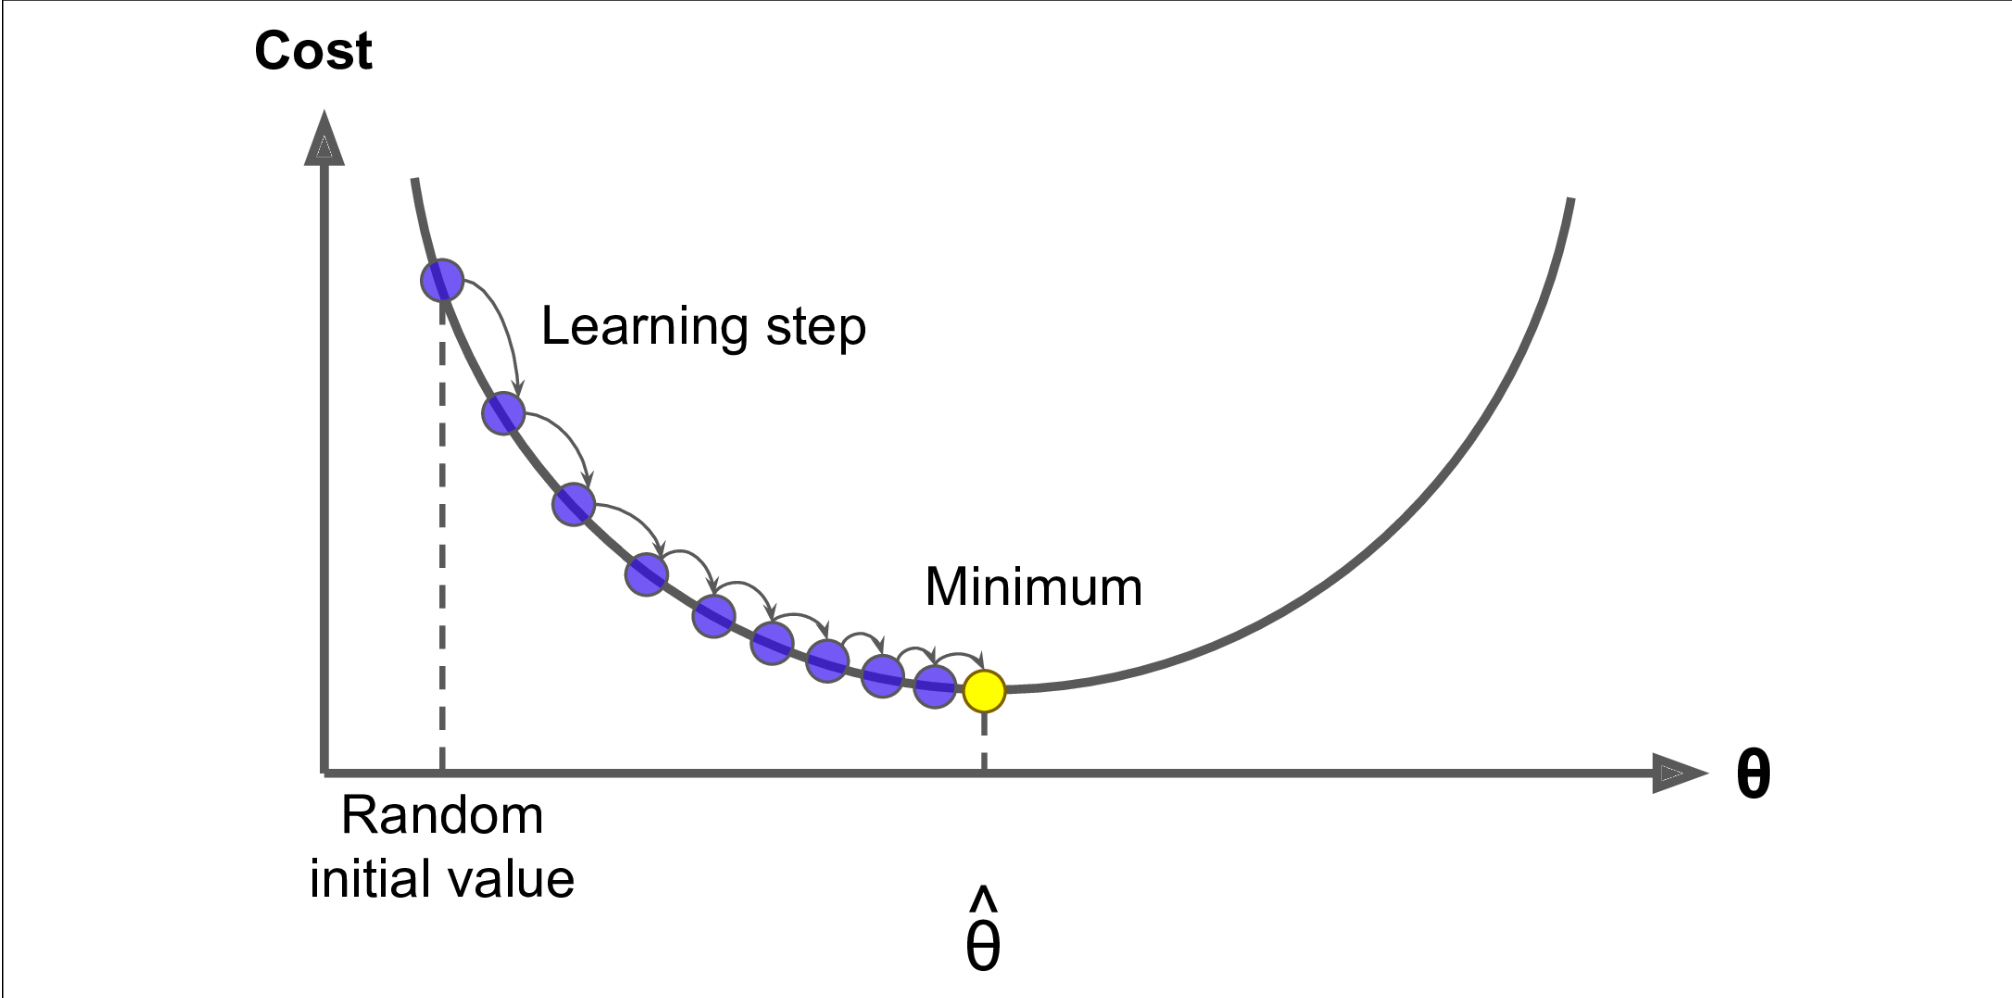
\includegraphics[scale=0.2]{GradientDescentNormal.jpeg}
    \caption{Gradient descent Normal Behavior\cite{Scikit-Learn}}
    \label{fig:normalbeh}
\end{figure}
\begin{figure}[htbp]
    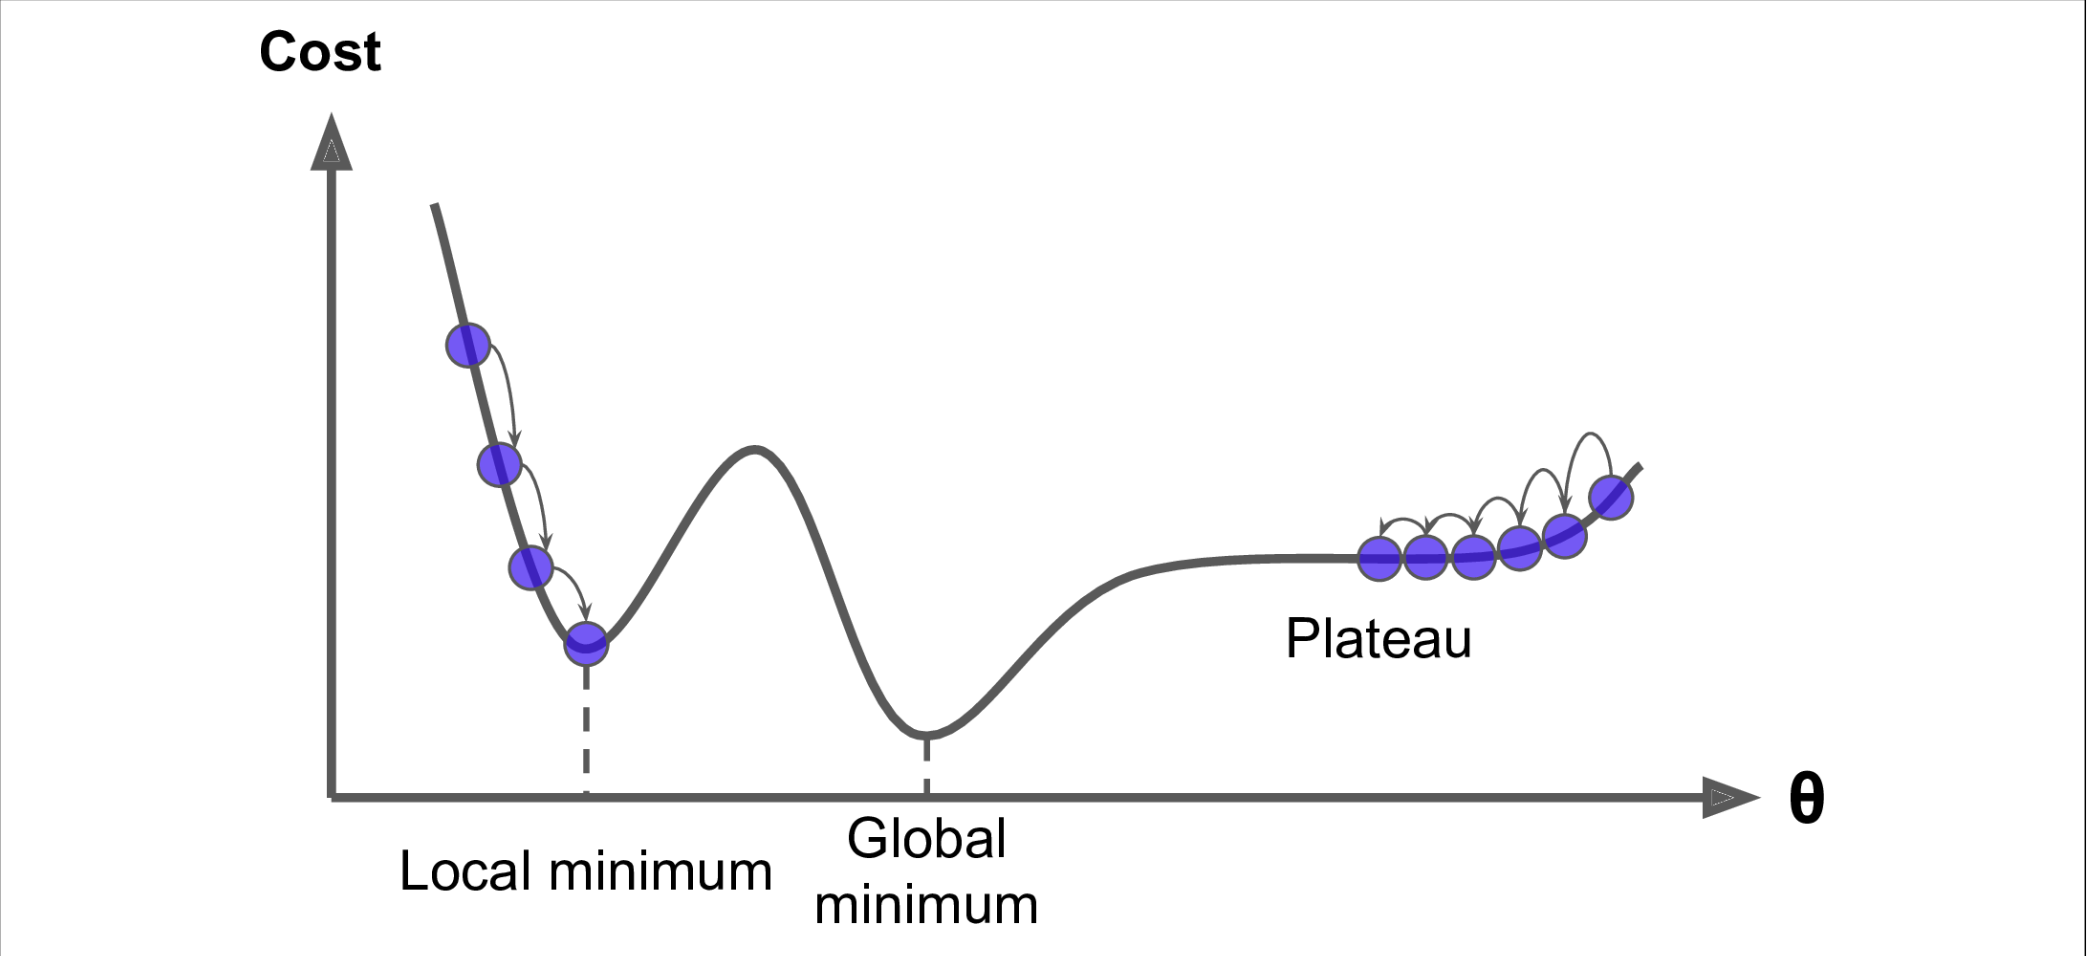
\includegraphics[scale=0.2]{GradientDescentPitfalls.png}
    \caption{Gradient descent pitfalls\cite{Scikit-Learn}}
    \label{fig:pitfallsbeh}
\end{figure}


\begin{figure*}[ht!]
     \begin{center}
        \subfigure[Gradient Descent Overshooting]{%
            \label{fig:first}
            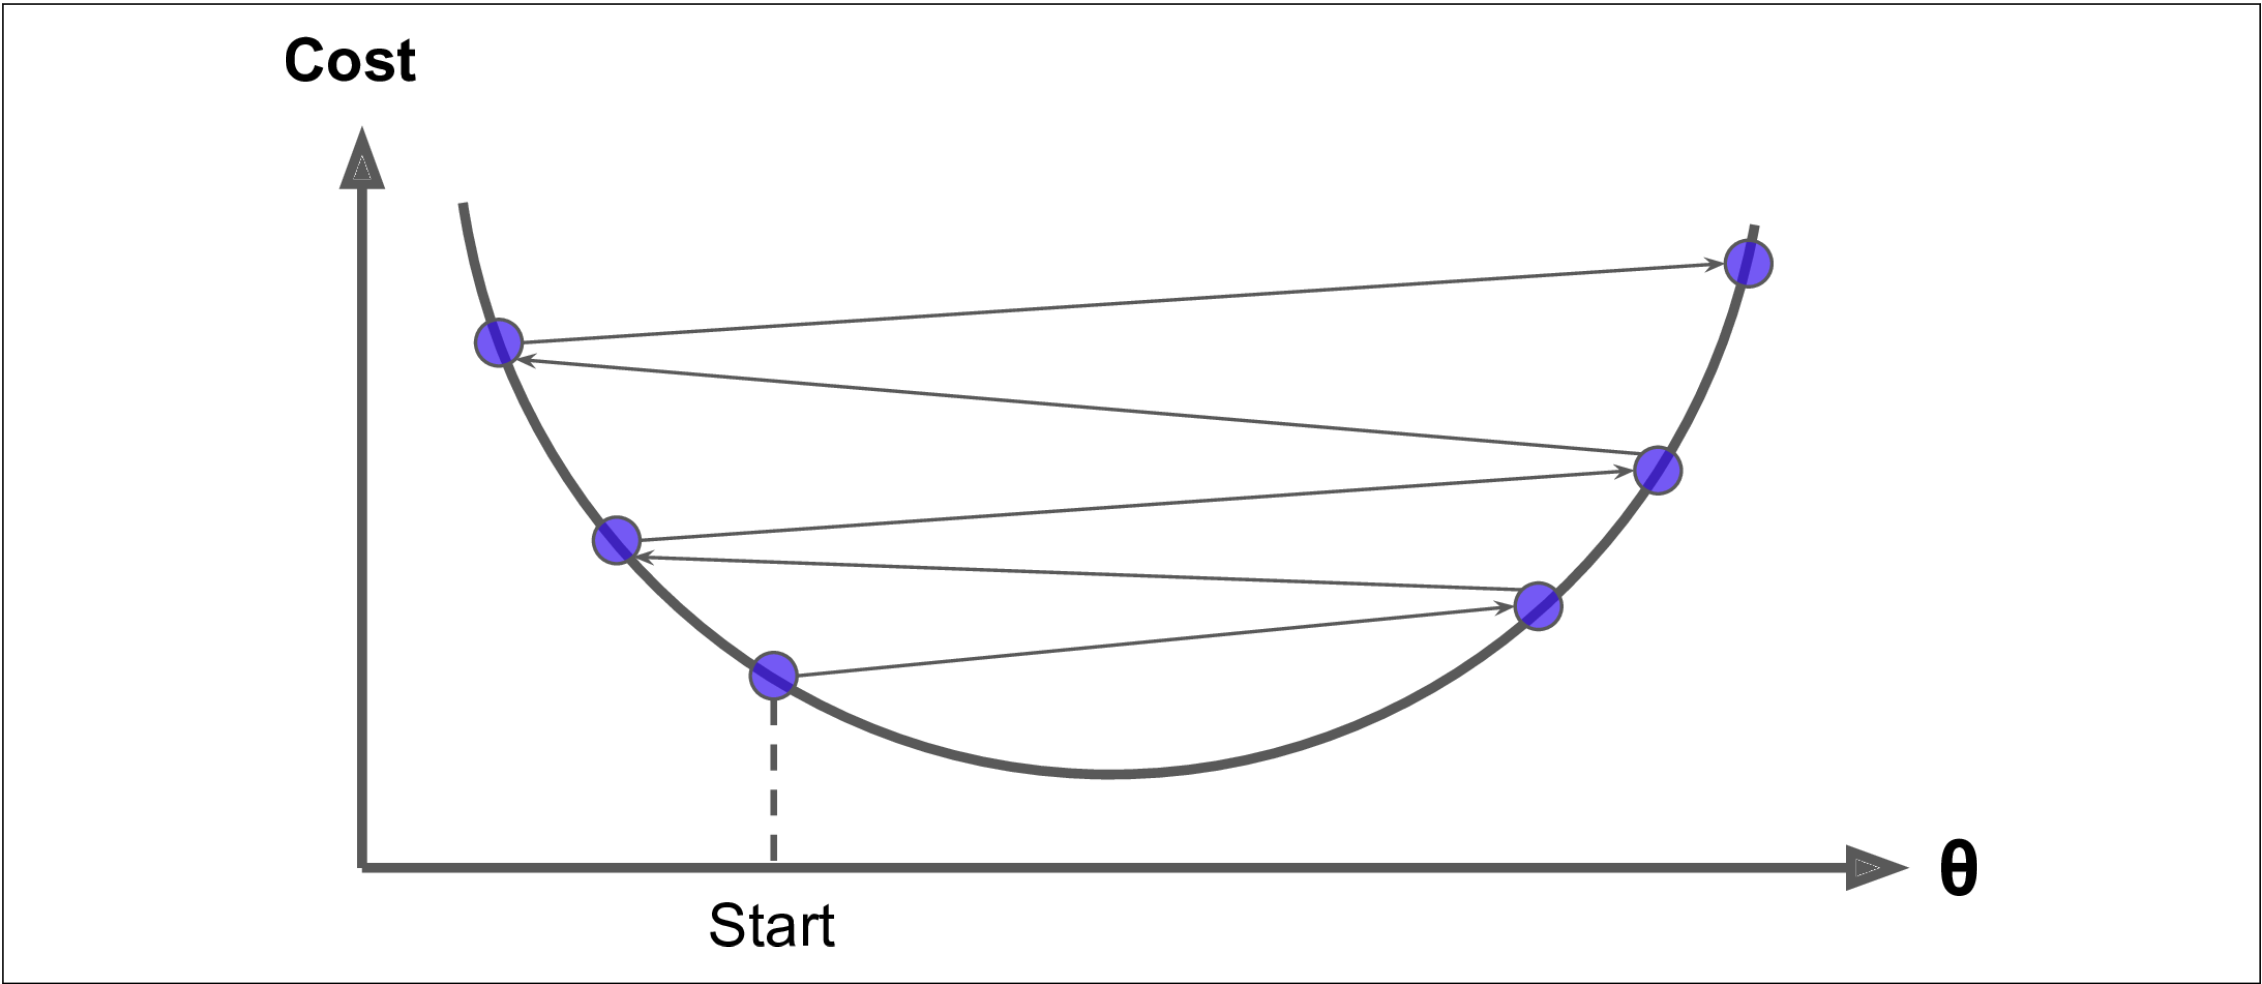
\includegraphics[scale = 0.2]{GradientDescentOvershoot.png}
        }%
        \subfigure[Gradient Descent using small steps]{%
           \label{fig:second}
           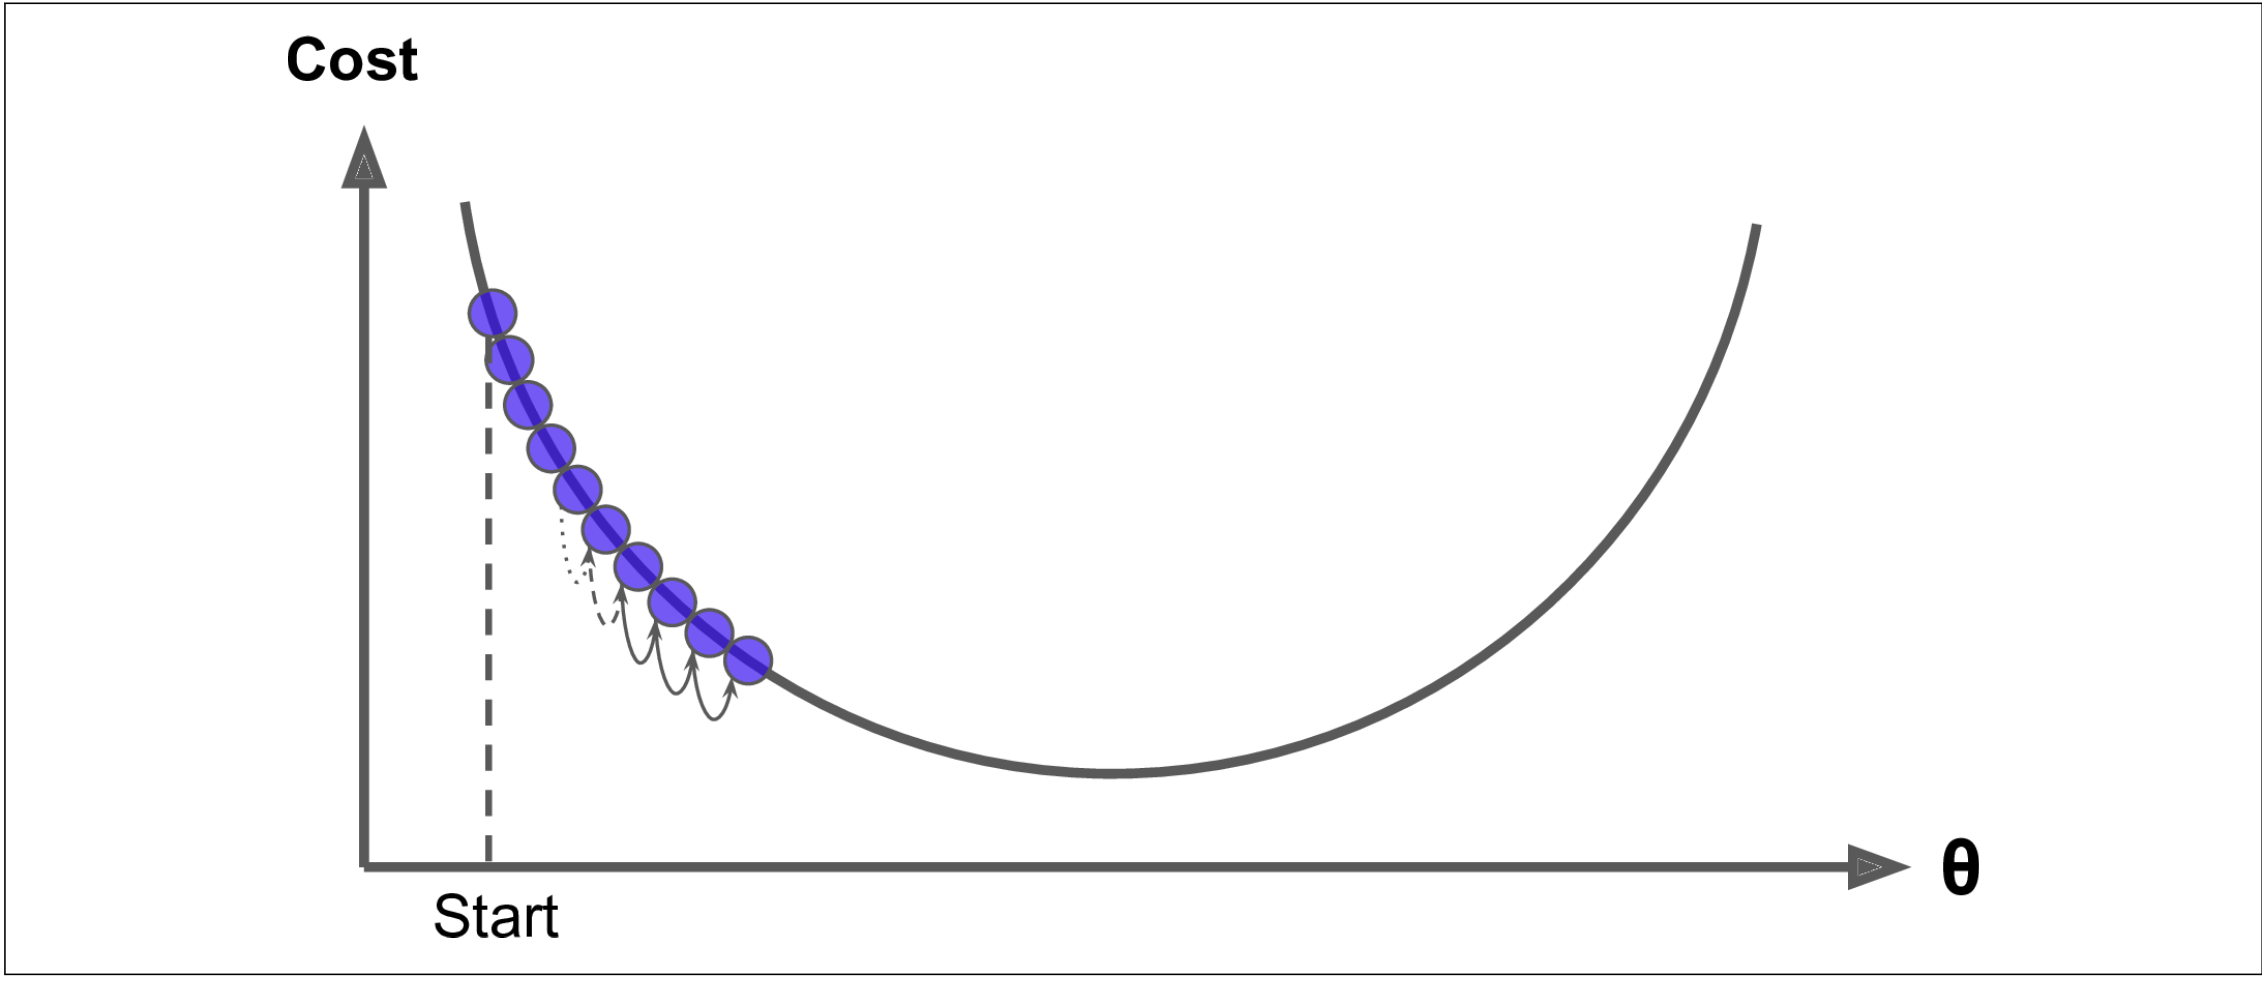
\includegraphics[scale = 0.2]{GradientDescentSmallSteps.png}
        }\\ %  ------- End of the first row ----------------------%
%
    \end{center}
    \caption{%
        Different behavior of the gradient descent with different type of learning rate\cite{Scikit-Learn}
     }%
   \label{fig:gradientbehavior}
\end{figure*}

\subsection{Development Environment}
An implementation example will be developed for all the versions of the algorithm using Python 3.9 and Scikit Learn 0.24.1. The data set called "Pima.tr" will be used to test the various implementation and it will be split beforehand into a training batch consisting of around 150 elements and a test batch of around 50. Fig n. \ref{fig:data_set} shows the data set. 
\begin{center}
    \begin{figure}[ht]
    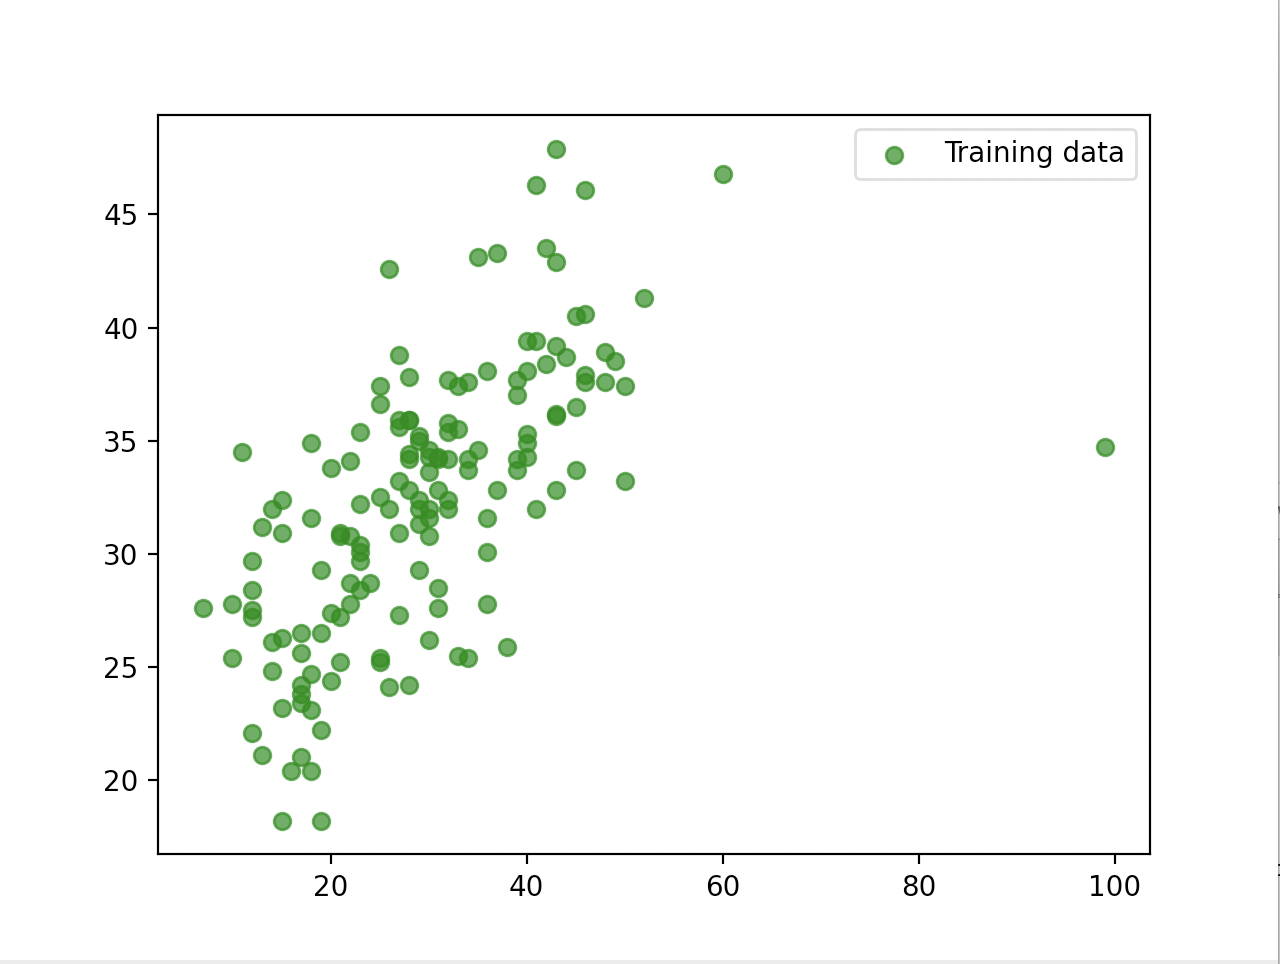
\includegraphics[scale=0.3]{Schermata 2021-05-11 alle 15.57.18.png}
    \caption{Training data set}
    \label{fig:data_set}
\end{figure}
\end{center}



\section{Batch Gradient Descent Application}
\subsection{Theory behind the algorithm}
The first variation of the algorithm is called Batch Gradient Descent Application, or Vanilla gradient descent, and can be thought as the naïve implementation of the algorithm.\cite{JZ2019} 
The idea of this algorithm is to translate the mathematical representation into code. 
Given a training set $\tau$, the \textit{Batch Gradient Descent algorithm} optimizes the model variables with the following equation:
\begin{equation}
    \Theta^{(i)} = \Theta^{(i-1)} -\alpha\nabla\mathscr{L}(\Theta;\tau)\label{BGDA}
\end{equation}
where:
\begin{enumerate}
  \item $\Theta^{(\tau)}$ denotes the model parameters vector at iteration $i$
  \item $\nabla\mathscr{L}(\Theta;\tau)$ denotes the gradient of the loss function $\mathscr{L}(\Theta;\tau)$.The notation $(\Theta;\tau)$ indicates that the parameters $\Theta$ are taken with the whole $\tau$. The loss function for the purpose of this paper will be defined as the Mean Squared Error (MSE) and will take the form of $\mathscr{L}(\Theta)= \frac{1}{N}\sum_{i=1}^{n}(\theta x_i - y_i)^2$.
  \item $\alpha$ denotes the  \textit{learning rate} in the gradient descent algorithm, which is usually very small (e.g. $10^{-4}$)
\end{enumerate}

The implementation of this type is described by Algorithm N.\ref{euclid}.

\begin{algorithm}
\caption{Vanilla Gradient Descent}\label{euclid}
\begin{algorithmic}[1]
\Require{Training set $\tau$, Learning Rate $\alpha$, Mean Squared Error(MSE): $\mathscr{L}(\Theta;\tau)$ }
\Ensure {Model Parameter $\theta$}
\For{i in $iterations$}\Comment{The amount of iterations is arbitrary }
\State Compute the gradient $\nabla\mathscr{L}(\theta;\tau)$
\State Update Variables $\Theta = \Theta -\alpha\nabla\mathscr{L}(\theta;\tau)$
\EndFor
\State \Return{model variable $\Theta$} \Comment{The vector $\Theta$ contains the update version of $w$ and $b$}
\end{algorithmic}
\end{algorithm}

The algorithm, however, can be optimized by working on Equation n. \ref{BGDA}.
Recalling that the loss function was defined as:
\[
\mathscr{L}(\Theta)= \frac{1}{N}\sum_{i=1}^{n}(\theta x_i - y_i)^2
\]
Let's find its derivative:

\[
\frac{d\mathscr{L}}{d\Theta} = \frac{2}{N}\sum_{i=1}^{n}x_i(\theta x_i - y_i)
\]
If we rewrite this in vector form, we find:

\begin{equation}
   \nabla\mathscr{L}(\Theta;\tau) = \begin{bmatrix}
            \nabla_{\Theta}\mathscr{L}(\Theta;\tau)_{1} \\
            \nabla_{\Theta}\mathscr{L}(\Theta;\tau)_{2} \\
           \vdots \\
            \nabla_{\Theta}\mathscr{L}(\Theta;\tau)_{m}
         \end{bmatrix} =  \frac{2}{N}\mathbf{\tau^{T}}(\mathbf{\tau\Theta}-\mathbf{y})
         \label{BGDAVF}
\end{equation}

Using \eqref{BGDAVF} the dot product is computed and it allows to compute all the partial derivatives in one go \cite{Scikit-Learn}.
Although this is faster than the previous one, the last formula will not solve the main problem of this version.
According to the description, using this variation of the algorithm, to update the model variables, the computation of the whole gradient of the loss function at every iteration is needed. This introduces computation overhead by redundancy which makes the training slow and does not allow online training. 

\subsection{Application}
In Fig \ref{fig:va_gr} a line-to-line implementation of the algorithm using python can be seen. This implementation is a revised implementation of the one found in \cite{Scikit-Learn}. The main difference is that \cite{Scikit-Learn} uses a random dataset, while this one is thought for the previously mentioned data set. 
\begin{figure}[ht]
    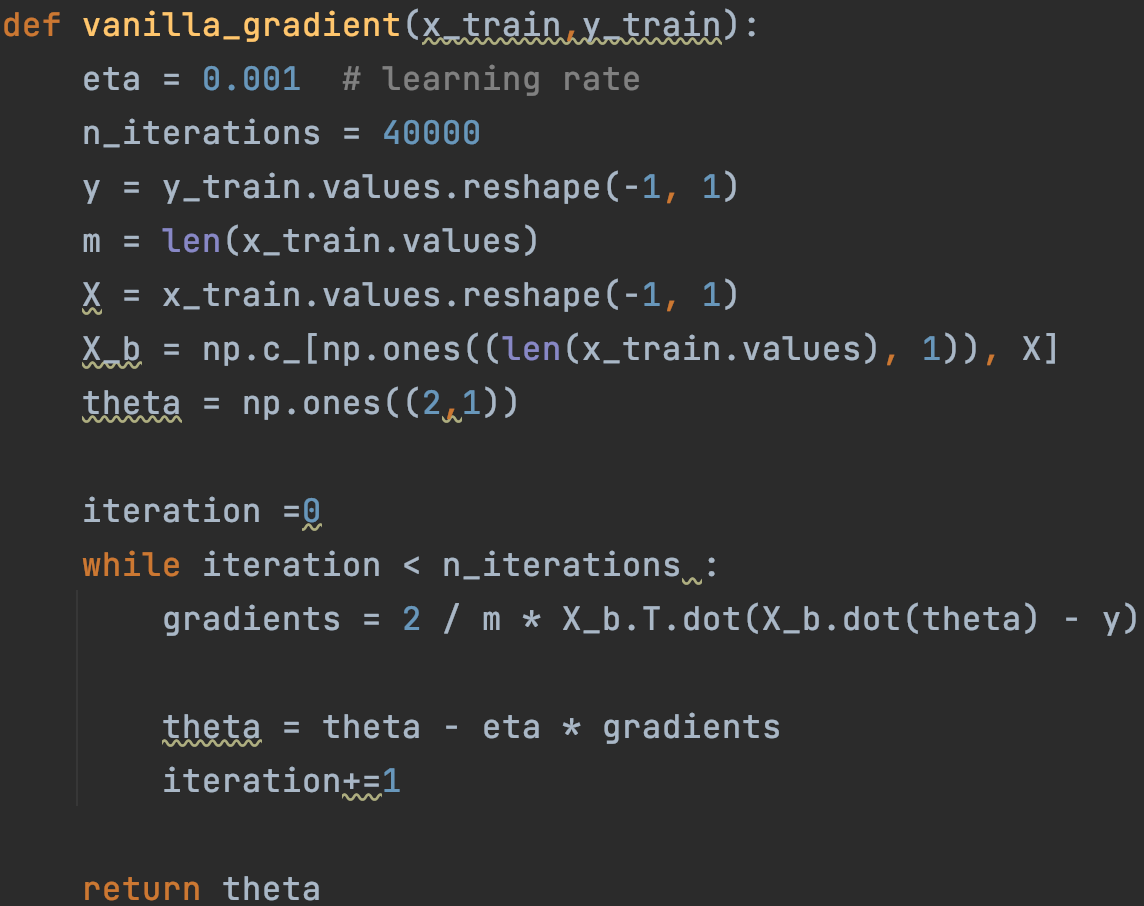
\includegraphics[scale=0.4]{vanilla_gradient.png}
    \caption{Implementation of the vanilla gradient descent in python}
    \label{fig:va_gr}
\end{figure}

\begin{figure}[ht]
    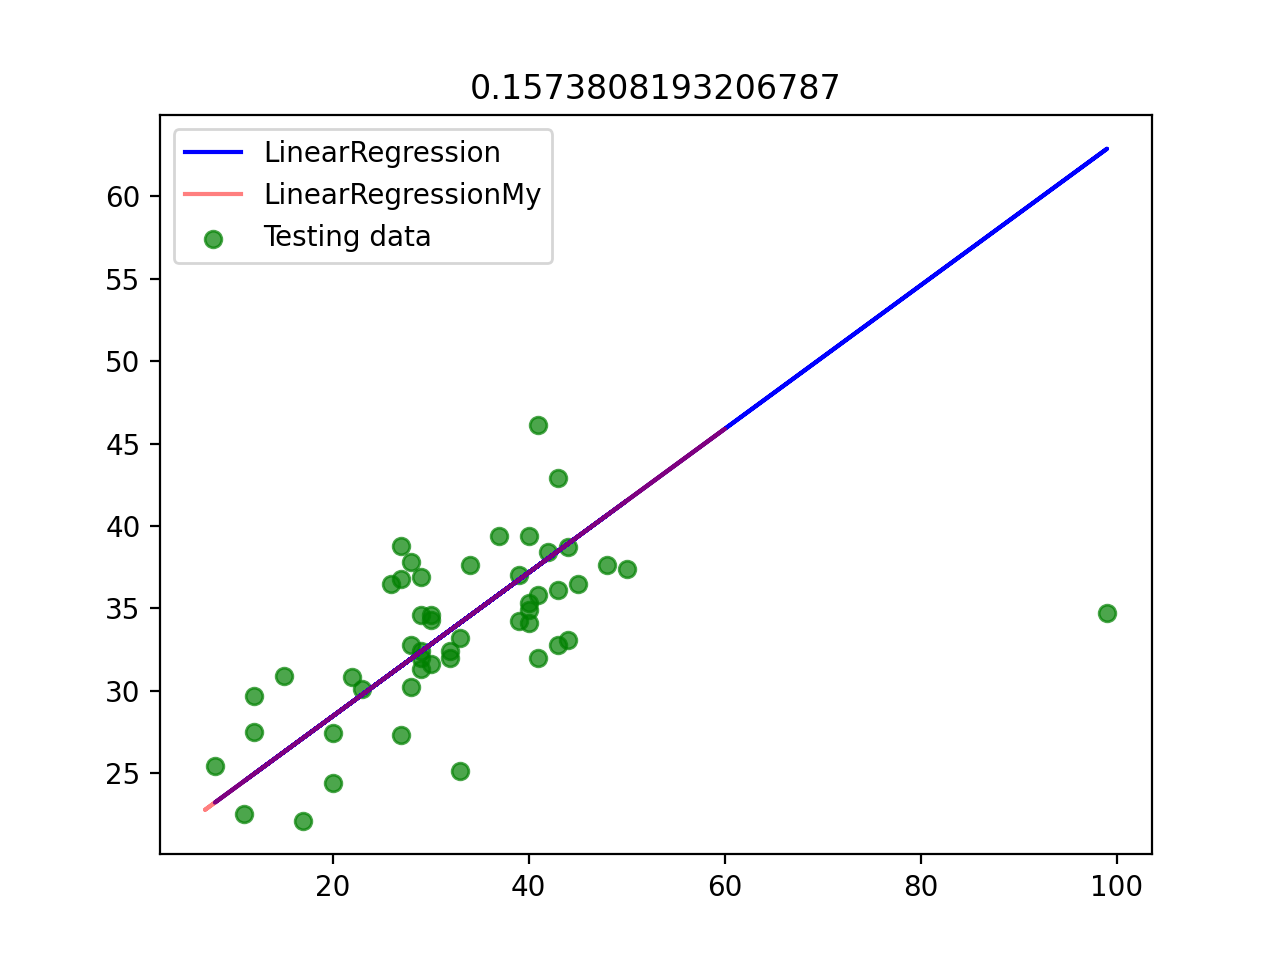
\includegraphics[scale=0.5]{Figure_1.png}
    \caption{Result of the implementation with a correct value of eta and the correct number of iterations}
    \label{fig:va_gr_ben}
\end{figure}
\subsection{Results}
The algorithm in Fig \ref{fig:va_gr} is measured against the standard implementation found in the Skilearn library. The result are compared in Fig \ref{fig:va_gr_ben}. On top of the graph the time taken by the algorithm is also shown.
The graph shows clearly that the two implementations produce the same model, however this is influenced heavily on the number of iterations and the eta chosen, which depend heavily on each other, as shown in Fig \ref{fig:va_gr_ben_eta_small} and Fig \ref{fig:va_gr_ben_eta_big}. 
In Fig \ref{fig:va_gr_ben_eta_small} an eta = 0.0001 is chosen. This means that a higher number of iterations (in this case around 16000) is needed to obtain a good enough model.\cite{Scikit-Learn} \\
This results in a longer time of execution (around 0.6709s compared to 0.1574s of the previous implementation). 
In Fig \ref{fig:va_gr_ben_eta_big} the result of the opposite case is shown. With an eta bigger than the proper one (eta = 0.001) the algorithm will not converge to a suitable value \cite{Scikit-Learn}, therefore only a few iterations are necessary to show that the model it produces (in this case, around 10) is not precise. As a result, the time of execution turns out to be lower as well (around 0.00015s).


\begin{figure}[ht]
    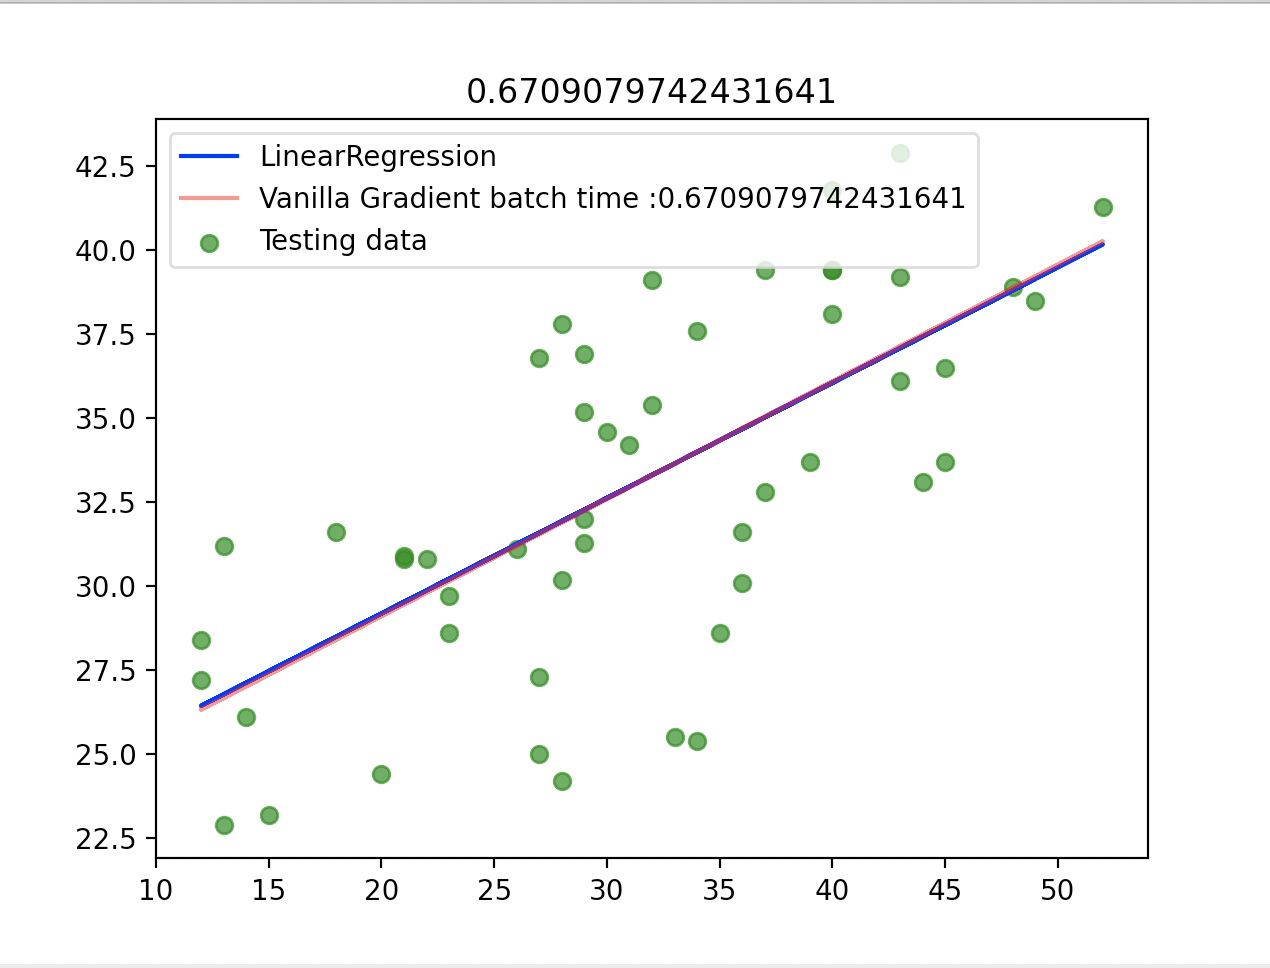
\includegraphics[scale=0.35]{Fig2.png}
    \caption{Result of the implementation with a small value for eta and a big number of iterations}
    \label{fig:va_gr_ben_eta_small}
\end{figure}


\begin{figure}[ht]
    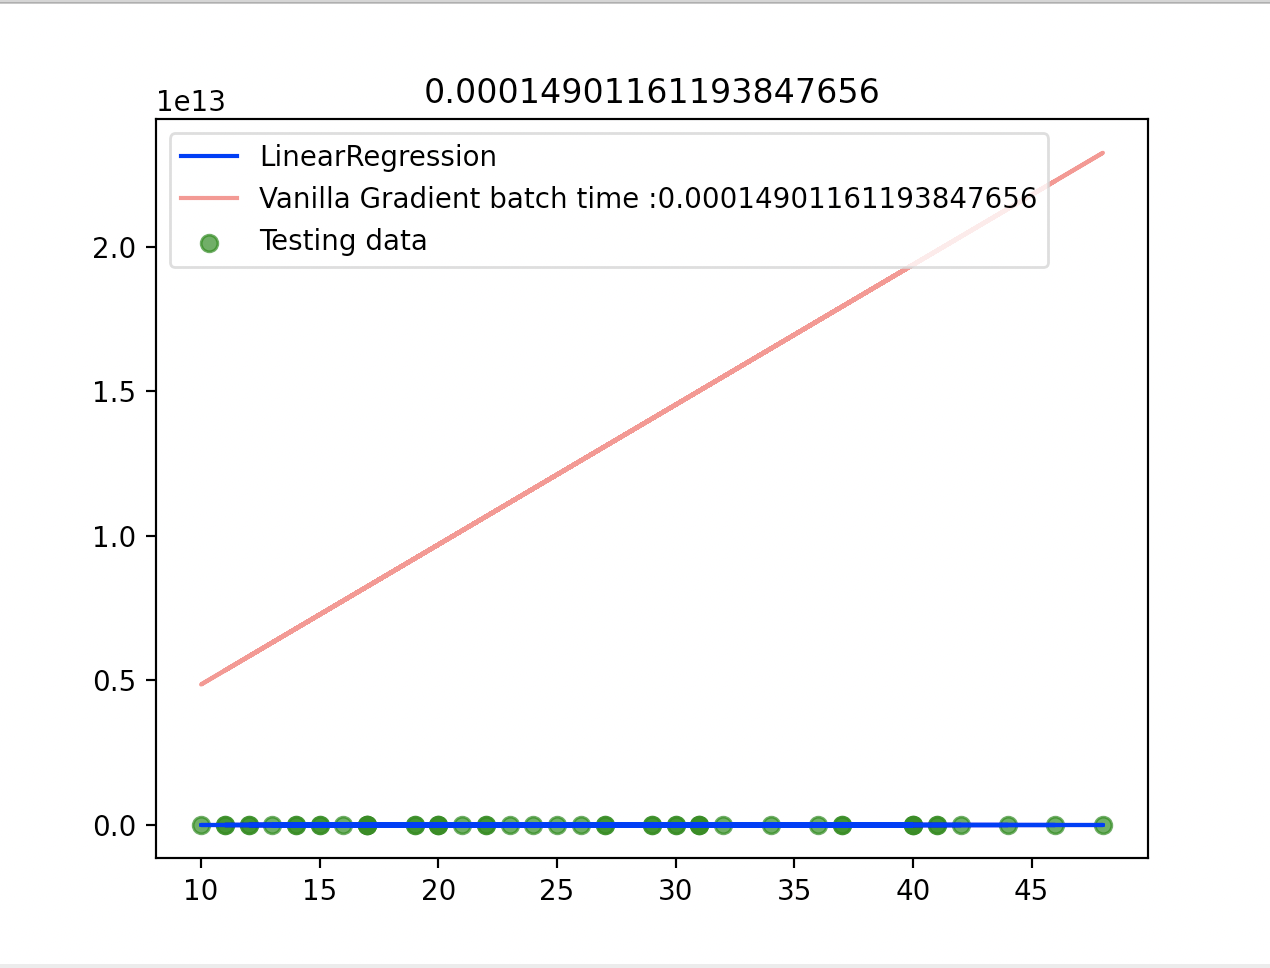
\includegraphics[scale=0.35]{Fig3.png}
    \caption{Result of the implementation with a big value for eta and a small number of iterations}
    \label{fig:va_gr_ben_eta_big}
\end{figure}


\subsection{Convergence Rate}
Since MSE is convex and does not change abruptly, the
Batch Gradient Descent with a fixed learning rate will eventually converge to the optimal solution. \\
In general, the algorithm takes 0(1/$\epsilon$) iterations to reach the  optimum within a range of $\epsilon$ depending on the shape of the cost function. By dividing the tolerance by N, the algorithm will need to run 10 times longer. \cite{Scikit-Learn}


\section{Stochastic Gradient Descent Application}

To improve efficiency, the \textit{Stochastic Gradient Descent Application} updates the parameters by computing the loss function gradient instance by instance. In other words, the gradient will be computed only once for every instance of our dataset. This means, equation \eqref{BGDA} will become:
\begin{equation}
    \Theta^{(i)} = \Theta^{(i-1)} - \alpha\nabla\mathscr{L}(\Theta;(x_i,y_i))\label{eq:SGDA}
\end{equation}
where:
%
\begin{enumerate}
  \item $\nabla\mathscr{L}(\Theta;(x_i,y_i))$ refers ot the gradient calculate at the point of the data set
\end{enumerate}
The pseudo code for this algorithm looks like algorithm n.\ref{SGDAal}. \\
\begin{algorithm}
\caption{Stochastic Gradient Descent Application}\label{SGDAal}
\begin{algorithmic}[1]
\Require{Training set $\tau$, Learning Rate $\alpha$, Mean Squared Error(MSE): $\mathscr{L}(\theta;\tau)$}
\Ensure {Model Parameter $\theta$}
\For{i in $iterations$}\Comment{The amount of iterations is arbitrary }
\State Shuffle $\tau$
\For{each instance $(x_i,y_i)\in \tau$}
\State Compute the gradient $\nabla\mathscr{L}(\theta;(x_i,y_i))$
\State Update Variables $\Theta = \Theta -\alpha\nabla\mathscr{L}(\Theta;(x_i,y_i))$
\EndFor
\EndFor
\Return{model variable $\Theta$}\Comment{The vector $\Theta$ contains the update version of $w$ and $b$}
\end{algorithmic}
\end{algorithm}
\begin{figure}[htbp]
    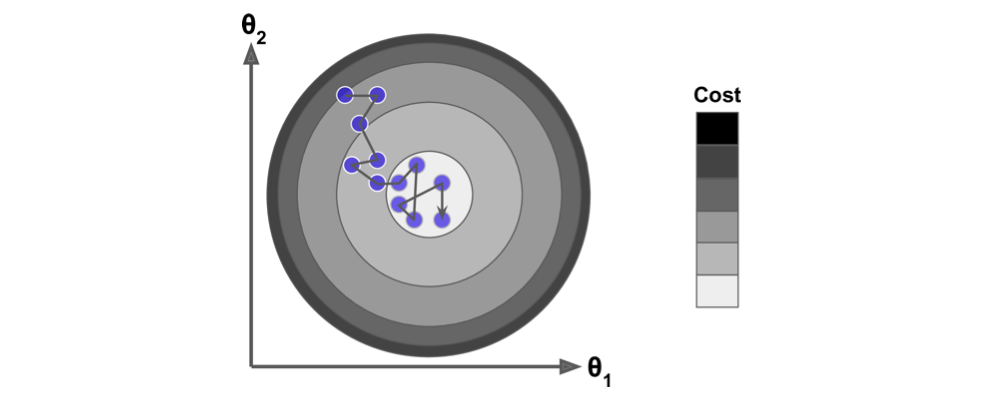
\includegraphics[scale=0.5]{Fig4.png}
    \caption{Concept of the stochastic gradient algorithm}
    \label{fig:st_grad}
\end{figure}
\\
While this implementation reduces the number of computations need, the main draw back is that, due to its randomness, is much less regular than Batch Gradient Descent: instead of gently decreasing until it reaches the minimum, the cost function will bounce up and down, decreasing only on average, as demonstrated in Fig n\ref{fig:st_grad}.
The possibility to overshoot and jump out of the local optimum is high,so\textit{Stochastic Gradient Descent Application} has a better chance of finding the global minimum than \textit{Batch Gradient Descent Application} does in case of a non convex function. 
Therefore randomness is good to escape from local optima, but bad because it means that the algorithm can never settle at the minimum. One solution to this dilemma is to gradually reduce the learning rate. The steps start out large (which helps make quick progress and escape local minima), then get smaller and smaller, allowing the algorithm to settle at the global minimum. This process is akin to simulated annealing, an algorithm inspired from the process of annealing in metallurgy where molten metal is slowly cooled down. The function that determines the learning rate at each iteration is called the learning schedule. If the learning rate is reduced too quickly, you may get stuck in a local minimum, or even end up frozen halfway to the minimum. If the learning rate is reduced too slowly, you may jump around the minimum for a long time and end up with a suboptimal solution if you halt training too early. \cite{Scikit-Learn}.


\subsection{Application}
The application of this variation of the algorithm uses the same data-set as the one before with surprising the results. 
According to  \cite{Scikit-Learn},  the two variations should give more or less the same result. This is probably the case when the data-set does not contain a lot of noise and it presents a pretty linear behavior. However, as shown in fig n. \ref{fig:data_set}, the data set used for this example contains a certain degree of noise that can influence the outcome of the algorithm. 
In addition, the stochastic gradient works better with non-convex, smooth error functions. The function used in this paper, as explained previously, is the MSE, which is a convex function, which means that if you pick any two points on the curve, the line segment joining them never crosses the curve. This implies that there are no local minima, just one global minimum. \cite{Scikit-Learn} This type of functions are not well suited to the randomness of such algorithm therefore unexpected results can come up. 
\begin{figure}[htbp]
    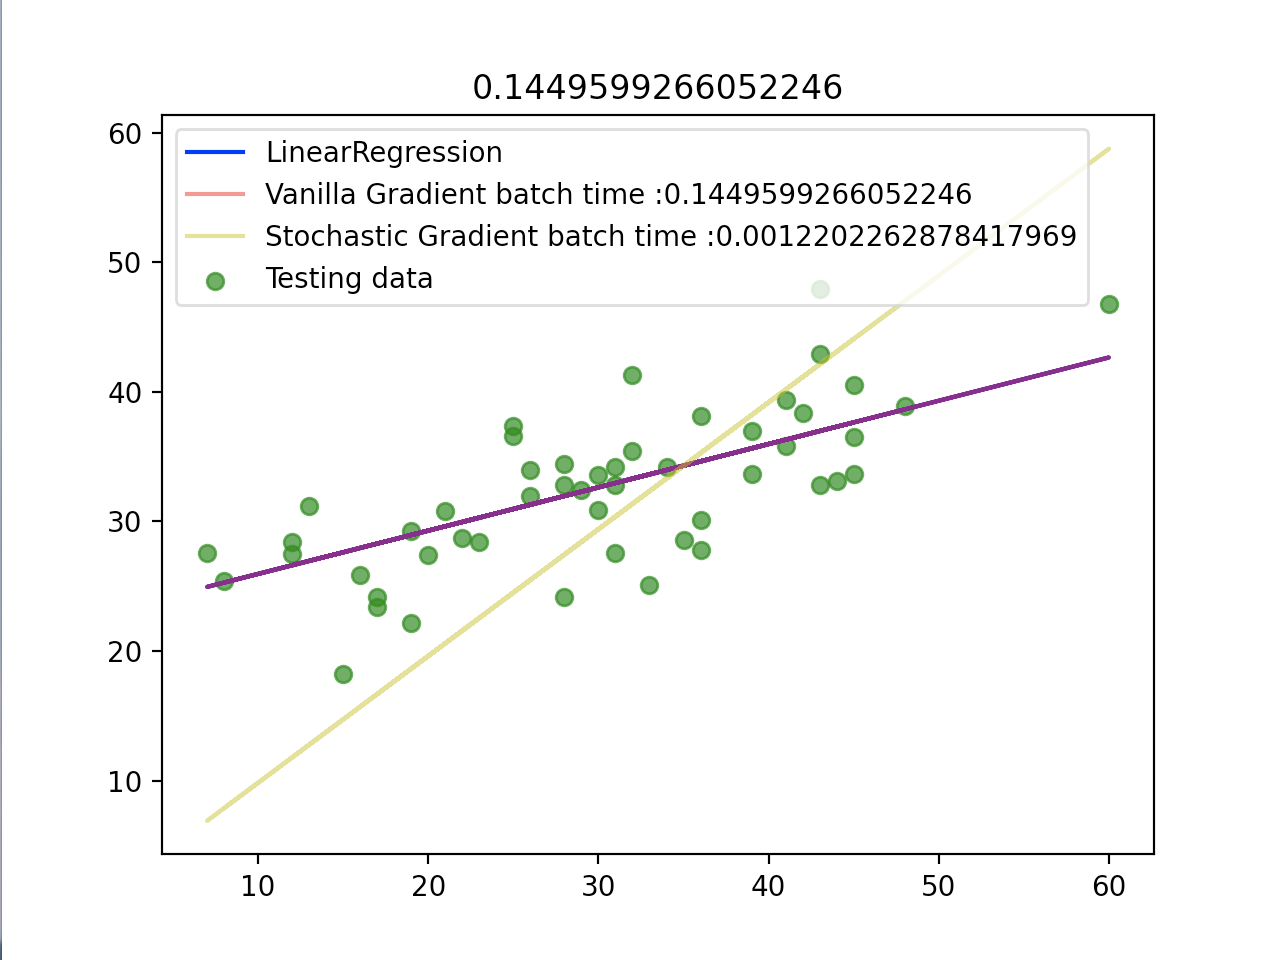
\includegraphics[scale=0.35]{Schermata 2021-05-01 alle 18.53.24.png}
    \caption{Result of the implementation of the stochastic gradient descent}
    \label{fig:stoc_res}
\end{figure}
The time needed by this version to come up with a behavioral model, however, is significantly less than the one needed by the vanilla gradient descent, as demonstrated in Fig n.\ref{fig:stoc_res}.




\section{Mini-Batch Gradient Descent Application}


To balance between the \textit{Vanilla Gradient Descent Application} and the  \textit{Stochastic Gradient Descent Application} an approach which lies in between the two can be taken. Instead of taken the whole dataset to compute the gradient, we can divided it in sub-sets called Mini Batch. This approach is therefore named \textit{Mini-Batch Gradient Descent}. \\
Formally, let $\beta \subset \tau$, we can rewrite \eqref{BGDA} as:
\begin{equation}
    \Theta^{(i)} = \Theta^{(i-1)} - \alpha\nabla\mathscr{L}(\Theta;\beta )\label{eq:MBGDA}
\end{equation}
With this newly obtained equation, the algorithm takes the form showed in algorithm n.\ref{MBGDA}.

\begin{algorithm}
\caption{Mini-Batch Gradient Descent Application}\label{MBGDA}
\begin{algorithmic}[1]
\Require{Training set $\tau$, Learning Rate $\alpha$, Mean Squared Error(MSE): $\mathscr{L}(\theta;\tau)$, Mini-batch size $b$}
\Ensure {Model Parameter $\theta$}
\For{i in $iterations$}
\State Shuffle $\tau$
\For{each sub-set $\beta \subset \tau$}
\State Compute the gradient $\nabla\mathscr{L}(\theta;\beta \subset \tau)$
\State Update Variables $\Theta = \Theta -\alpha\nabla\mathscr{L}(\Theta;\beta \subset \tau)$
\EndFor
\EndFor
\Return{model variable $\Theta$}
\end{algorithmic}
\end{algorithm}
In the \textit{Mini-batch Gradient Descent Application}, the mini batches are usually sampled sequentially from $\tau$, which means that $\tau$ is divided in multiple subsets of size b\footnote{b should not be very large, usually 64,256 or 128}, and these batches are picked one by one to train the model. Some versions select the batches randomly and this is referred to as the random mini-batch generation process.Compared with vanilla gradient descent, the mini-batch gradient descent algorithm is much more efficient especially for the training set of an extremely large size. Meanwhile, compared with the stochastic gradient descent, the mini-batch gradient descent algorithm greatly reduces the variance in the model variable updating process and can achieve much more stable convergence.\cite{JZ2019} It should also be noted that this variation still contains randomness, thus carrying the same drawbacks that the normal stochastic approach has. 
\begin{figure}[htbp]
    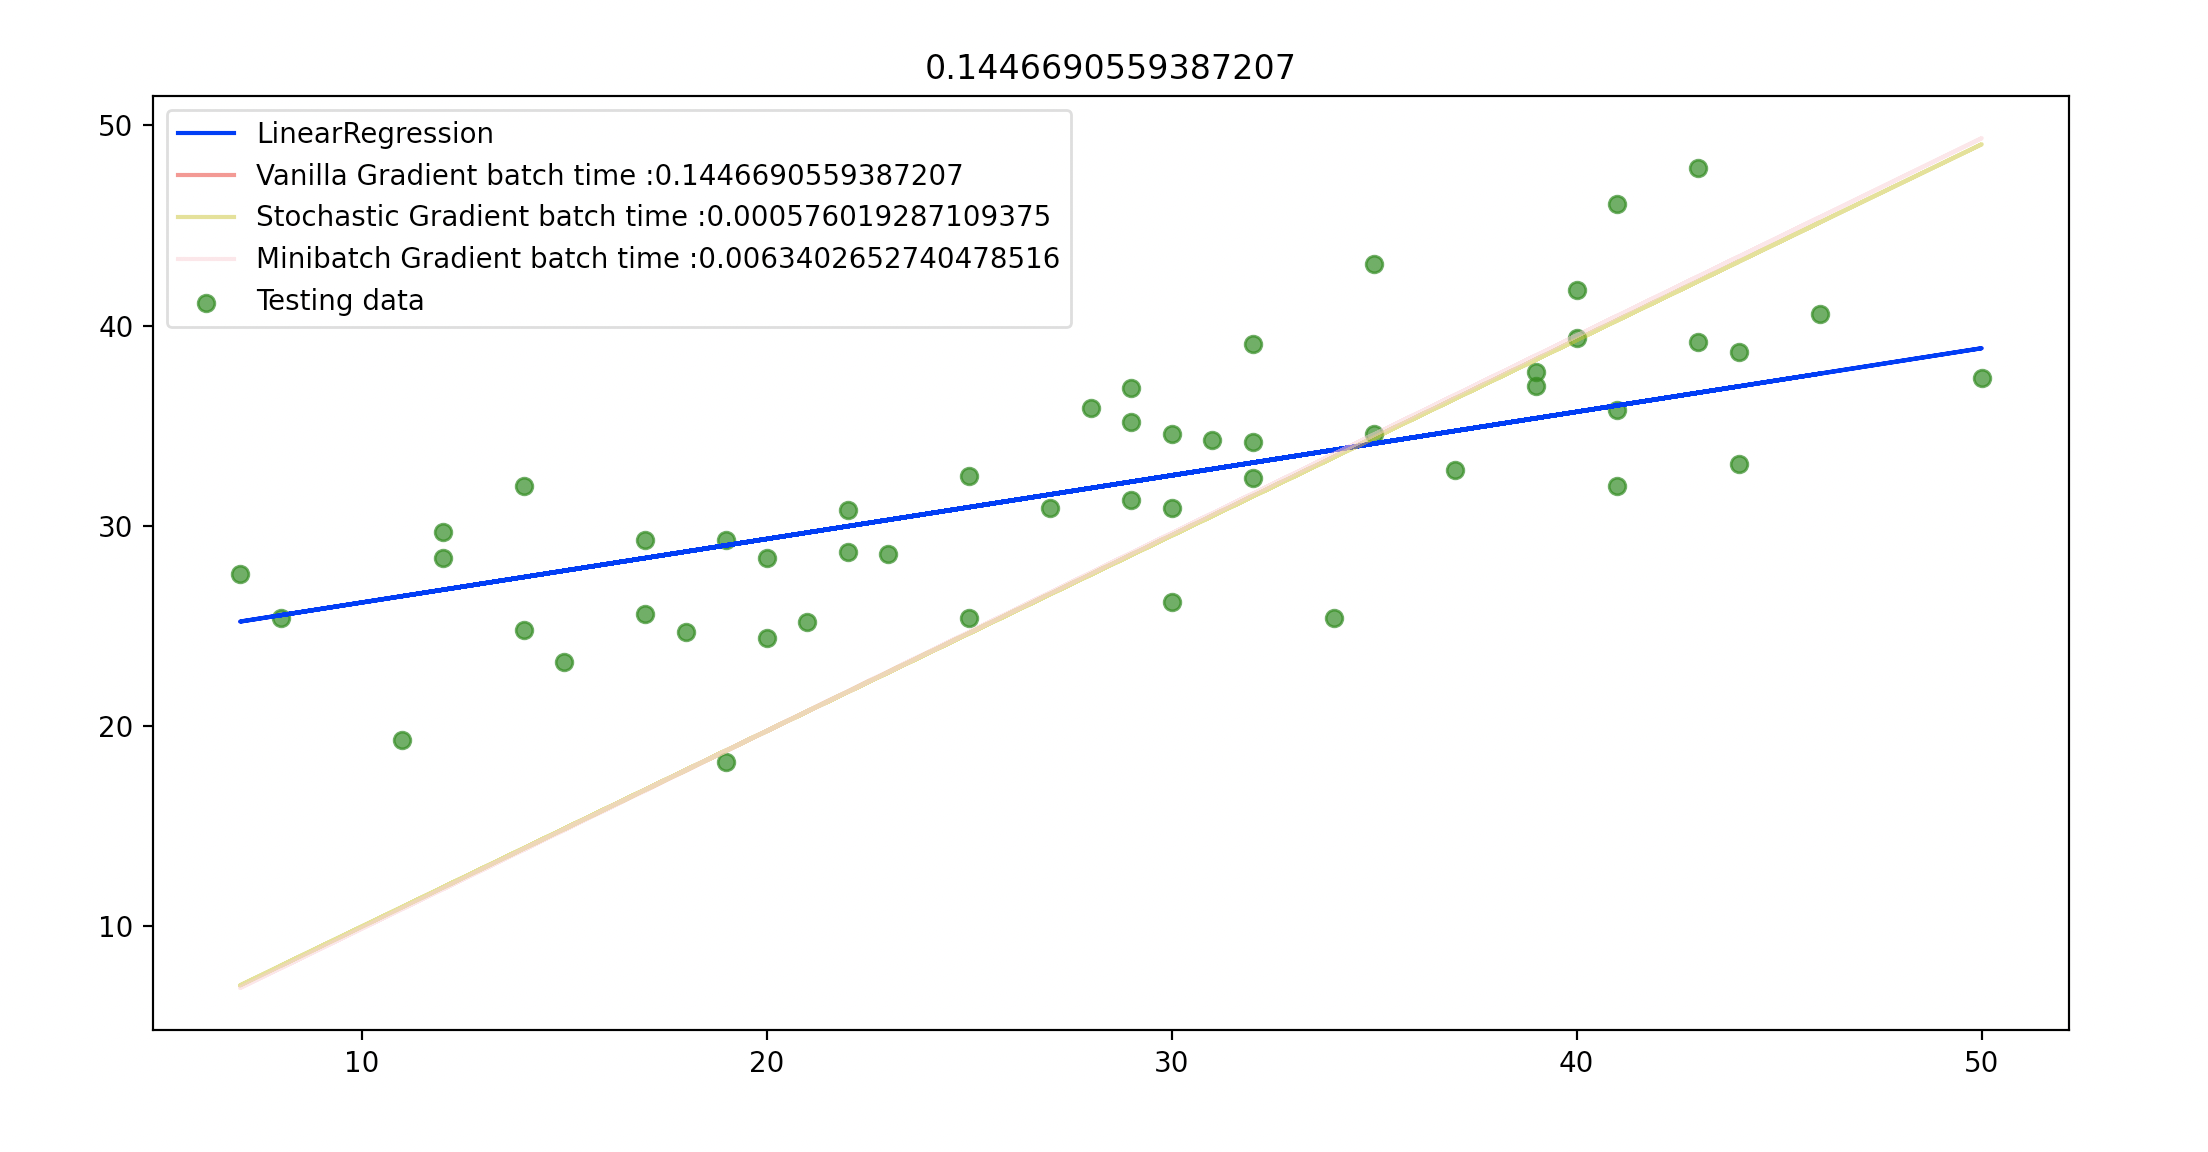
\includegraphics[width = 9 cm]{Schermata 2021-05-11 alle 16.25.08.png}
    \caption{Result of the mini batch gradient descent algorithm}
    \label{fig:mini_res}
\end{figure}


\subsection{Application}
Fig n.\ref{fig:mini_res} shows the result of the Mini-Batch algorithm.As expected,the result matches the one with the stochastic method. This shows that this variation is not well-suited for a convex error function as well. 
It was also to be expected,that the time of execution is would be a bit higher than the stochastic version(around 0.0063s compared to around 0.0005s), but still to be considered an improvement over the vanilla approach. 








\section{Conclusion}

In this paper we have explored the Gradient Descend algorithm with its variations for optimizing learning models. The Gradient descend is a very popular algorithm in the field of machine learning but, in its vanilla form, tends to be particularly slow, since it iterates through the whole data set. To obviate to this problem, a stochastic, e.g. random, approach is used. Either a single instance of the data set, in the case of the Stochastic Gradient Descent, or a subsets of the data set, in the case of the Mini-Batch Gradient Descent, are chosen at every iteration to compute the gradient. If on the one hand, this approach allows the learning process to speed up, on the other hand, it also reduces precision if a not-suitable error function is chosen. 
\cite{Scikit-Learn} offers a good comparison between the three variations and it can be seen in Fig n.\ref{fig:comparison}.
The Vanilla Gradient descent, or "Batch", converges smoothly towards the minimum value of the function, while the stochastic and mini-batch ones tend to over-shoot and never to settle into a proper minimum. This is due to their more random nature. These two last variations, however,  tend to reach the zone of the minimum faster, i.e. with less iterations and less computational overhead. 
This is the trade-off that needs to be considered when choosing one of the variations and it is necessary to know all of them to optimize the learning process. 
\begin{figure}[htbp]
    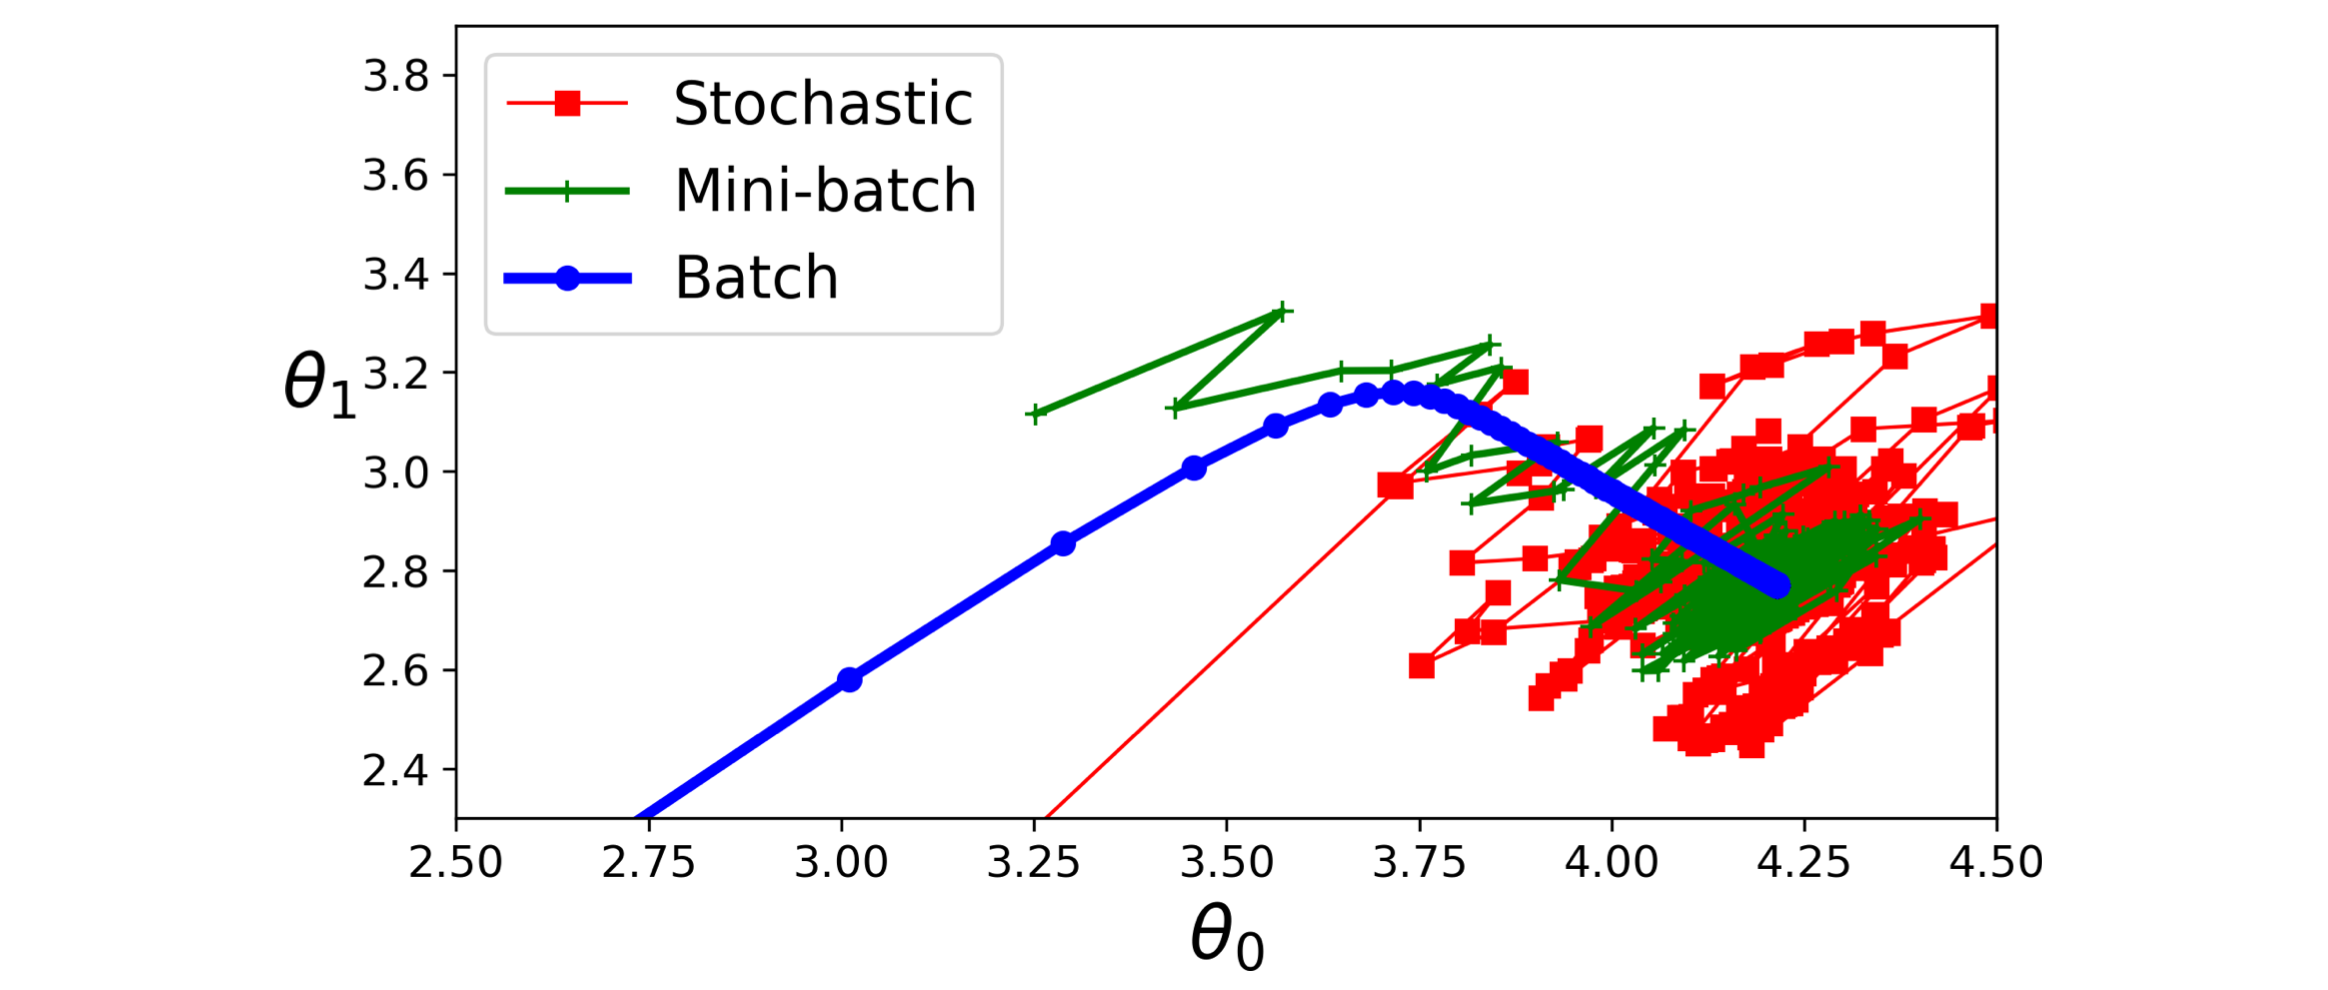
\includegraphics[width = 10cm]{Schermata 2021-05-11 alle 16.26.13.png}
    \caption{Comparison between the 3 variations}
    \label{fig:comparison}
\end{figure}

\newpage

\section{Declaration of Originality}
I hereby confirm that I have written the accompanying paper by myself, without contributions from any sources other than those cited in the text and acknowledgements.
This applies also to all graphics, drawings, maps and images included in the paper.
The paper was not examined before, nor has it been published.

\bibliographystyle{plain}
\bibliography{mybibfile} 


\end{document}